13. Введём систему координат с центром в левом нижнем угле прямоугольника. Тогда диагональ --- это прямая $y=\cfrac{239}{566}x.$ Она не проходит ни через один узел сетки внутри прямоугольника, так как в таком случае и $x,$ и $y$ были бы целыми числами что невозможно, так как $x<566$ и $\text{НОД}(239,566)=1,$ поэтому домножение на $x$ не сможет сократить полностью знаменатель. Значит, диагональ пересекает по 1 разу в разных точках все вертикальные прямые $x=1,\ 2,\ \ldots 566$ и горизонтальные прямые $y=1,\ 2,\ \ldots 239,$ за исключением последней точки, правой верхней вершины прямоугольника. Последняя точка считается два раза, поэтому всего точек пересечения $566+239-1=804.$ Каждой точке пересечения можно сопоставить ту клетку, в которой диагональ находилась перед пересечением (будем считать, что мы двигаемся вправо-вверх), тогда диагональ пересекает 804 клетки.
\begin{figure}[ht!]
\center{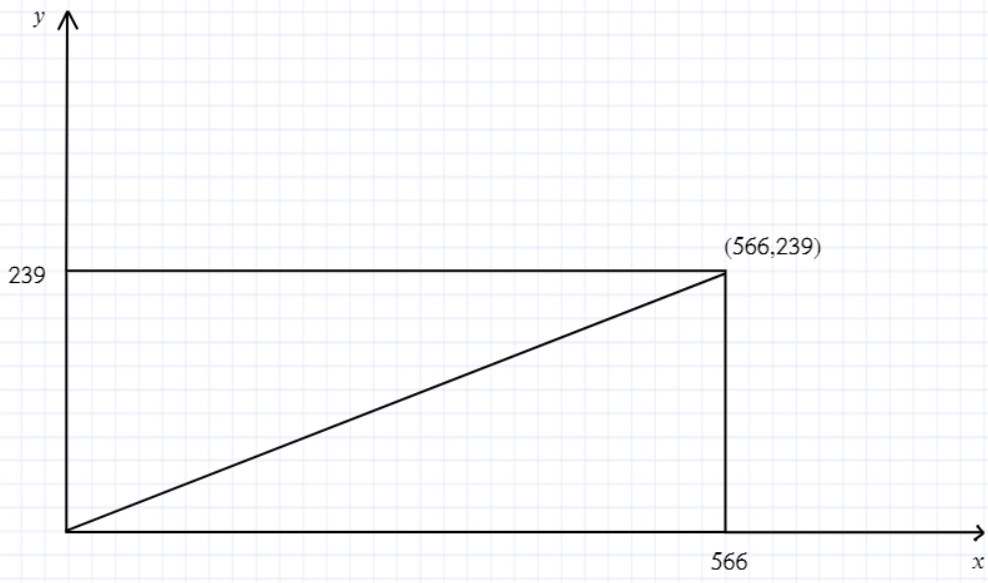
\includegraphics[scale=0.25]{566.png}}
\end{figure}\\
